\documentclass{article}
\usepackage[margin=1in]{geometry}      % default margins are too big
\usepackage{graphicx}                  % for \includegraphics
\usepackage{listings}                  % for typesetting source code
\lstset{language=Python}
\usepackage{mathtools}                 % for better typesetting of math
%\usepackage[round]{natbib}                    % for using different bibliography styles
\bibliographystyle{ieeetr}  
\usepackage{url}
%\usepackage{amsmath}

\usepackage{caption}
\usepackage{subcaption}
\usepackage{listings}
\usepackage{color}

\definecolor{dkgreen}{rgb}{0,0.6,0}
\definecolor{gray}{rgb}{0.5,0.5,0.5}
\definecolor{mauve}{rgb}{0.58,0,0.82}

\lstset{frame=tb,
  language=Java,
  aboveskip=3mm,
  belowskip=3mm,
  showstringspaces=false,
  columns=flexible,
  basicstyle={\small\ttfamily},
  numbers=none,
  numberstyle=\tiny\color{black},
  keywordstyle=\color{black},
  commentstyle=\color{black},
  stringstyle=\color{black},
  breaklines=true,
  breakatwhitespace=true
  tabsize=3
}                 % for typesetting source code

\begin{document}

\title{Implementation Report-2\\
using Reinforcement Learning to create Offloading Decision Engine}

\author{Aditya Khune}
\date{\today}  % Leave this line out to use the current date.
\maketitle

%%%%%%%%%%%%%%%%%%%%%%%%%%%%%%%%%%%%%%%%%%%%%%%%%%%%%%%%%%%%%%%%%%%%%%

\tableofcontents

%%%%%%%%%%%%%%%%%%%%%%%%%%%%%%%%%%%%%%%%%%%%%%%%%%%%%%%%%%%%%%%%%%%%%%
% Abstract wont come in table of contents! 2

\begin{abstract}
In this report I have explored Reinforcement Learning to create a decision engine prototype for the offloading process. Reinforcement learning is learning by interacting with an environment. Reinforcement Learning (RL) differs from standard supervised learning in that correct input/output pairs are never presented. 
\par
I have explained how the offloading decision process can benefit from Reinforcement Learning and also presented different scenarios where it can be applicable. I have referred the research in Reinforcement Learning which being used today in Computer Games for instance chess, tic-tac-toe, etc. I have developed a code in Python to demonstrate the prototype of the Reinforcement Learning offloading app engine.
\end{abstract}

%%%%%%%%%%%%%%%%%%%%%%%%%%%%%%%%%%%%%%%%%%%%%%%%%%%%%%%%%%%%%%%%%%%%%%

\section{Introduction}
Reinforcement learning is learning by interacting with an environment. An RL agent learns from the consequences of its actions, rather than from being explicitly taught and it selects its actions on basis of its past experiences (exploitation) and also by new choices (exploration), which is essentially trial and error learning. The reinforcement signal that the RL-agent receives is a numerical reward, which encodes the success of an action's outcome, and the agent seeks to learn to select actions that maximize the accumulated reward over time.\par
A reinforcement learning engine interacts with its environment in discrete time steps. At each time t, the agent receives an observation $O_t$, which typically includes the reward $r_t$. It then chooses an action $a_t$ from the set of actions available, which is subsequently sent to the environment. The environment moves to a new state $s_{t+1}$ and the reward $r_{t+1}$ associated with the transition $(s_t,a_t,s_{t+1})$ is determined. The goal of a reinforcement learning agent is to collect as much reward as possible. The agent can choose any action as a function of the history and it can even randomize its action selection.  \par
Reinforcement learning is particularly well suited to problems which include a long-term versus short-term reward trade-off. It has been applied successfully to various problems, including robot control, elevator scheduling, telecommunications, etc. \par
The basic reinforcement learning model consists of:
\begin{itemize}
    \item a set of environment states $S$;
    \item a set of actions $A$;
    \item rules of transitioning between states;
    \item rules that determine the scalar immediate reward of a transition
\end{itemize}

\begin{figure}[h]
  \centering
  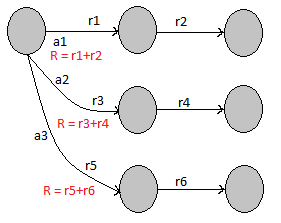
\includegraphics[width=2in]{RL.png}
  \caption{Choose from available actions with best Reinforcement History}
  \label{fig:RL}
\end{figure}

We want to choose the action that we predict will result in the best possible future from the current state in Figure~\ref{fig:RL}. Need a value that represents the future outcome. With the correct values, multi-step decision problems are reduced to single-step decision problems. Just pick action with best value and its guaranteed to find optimal multi-step solution! The utility or cost of a single action taken from a state is the reinforcement for that action from that state. The value of that state-action is the expected value of the full return or the sum of reinforcements that will follow when that action is taken.\par
Say we are in state $s_t$ at time $t$. Upon taking action $a_t$ from that state we observe the one step reinforcement $r_{t+1}$, and the next state $s_{t+1}$. Say this continues until we reach a goal state, $K$ steps later we have return as:
 \begin{align*}
      R_t = \sum_{k=0}^K r_{t+k+1}
  \end{align*}
So the aim of Reinforcement Learning algorithm generally is either to maximize or minimize the reinforcements $R_t$ depending upon our Reinforcement function.
%%%%%%%%%%%%%%%%%%%%%%%%%%%%%%%%%%%%%%%
\section{Proposed Mechanism}
A function called $Q$ function stores the reinforcement values for each case it encounters, some more mathematics about this $Q$ function which is used in RL algorithm is shown here:
\subsection{Q Function}
The state-action value function is a function of both state and action and its value is a prediction of the expected sum of future reinforcements. We will call the state-action value function $Q$.
\begin{align*}
      Q(s_t,a_t) \approx \sum_{k=0}^\infty r_{t+k+1}
\end{align*}

here $s_t$ = state, $a_t$ = actions, and $r_t$ = reinforcements received.
This is usually formulated as the least squares objective:


    \begin{align*}
      \text{Minimize } \mathrm{E} \left ( \sum_{k=0}^\infty r_{t+k+1} - Q(s_t,a_t)\right )^2
    \end{align*}
    

%%%%%%%%%%%%%%%%%%%%%%%%%%%%%%%%%%%%%%%
\subsection{The Idea}
Now let's consider the number of battery units consumed by our smartphone as our reinforcements. If we can minimize these units then we achieve reduction in the battery consumption! very intuitive right? \par
We need following things to train the Q function:
\begin{itemize}
   \item action selection
   \item state transitions
   \item reinforcement received
\end{itemize}
The State of the function in our case can hold parameters such as: Bandwidth, Data required by application, WiFi availability, Location of the device etc. The actions in this mechanism can be Offload, Do Not Offload, or Offload at a specific server. And finally reinforcements can be Battery Units consumed.\par

%%%%%%%%%%%%%%%%%%%%%%%%%%%%%%%%%%%%%%%%%%%%%%%%%%%%%%%%%%%%%%%%%%%%%%
\section{Implementation and Results}

\subsection{Scenario 1}
In this scenario I have considered the parameters that I had used to create a fuzzy logic decision engine in my earlier Implementation report \cite{adityaFL}. Consider an application for which we want to train the $Q$ function for various instances of following parameters:
\begin{itemize}
   \item Bandwidth = Speed Low, Speed Normal, Speed High
   \item WiFi = available, not available
   \item Data transfered = Data Small, Data Medium, Data Big
   \item CPU instance = CPU Low, CPU Normal, CPU High
\end{itemize}

We need to train our $Q$ function in all these conditions. In each such instance our smartphone will have three actions to choose from which are
\begin{itemize}
   \item Local Processing
   \item Offload on Local Servers
   \item Offload on Remote Servers
\end{itemize}
After choosing any of these actions, the smartphone will record the battery units consumed during the processing of the application. The reinforcements will be assigned depending upon the battery consumption. The action which gave us best performance will be the one which consumed least battery units. So we are minimizing our battery units consumption here.\par

\subsubsection{Code}
I have developed a Python code to demonstrate this algorithm. As I do not have a real time app running on smartphone for this instead of using Reinforcements as actual battery units, we will assign reinforcements based on an Ideal situation of offloading. Let us look into some snippets of the code. In the function printParameters(board) shown below we can specify the parameters that we want to consider for training our Q function.
\begin{small}
\begin{lstlisting}
def printParameters(board):
    print(```
bandwidth= {} |Data= {} |CPU_Instance= {} |Wifi= {}
'''.format(*tuple(board)))
\end{lstlisting}
\end{small}

The epsilonGreedy function helps us choose our actions randomly in the initial trials and after sufficient trials we decay the value of epsilon to take the `greedy' move that means to choose the action for which our Q function shows best reinforcement.
\begin{small}
\begin{lstlisting}
def epsilonGreedy(epsilon, Q, board, Out):
    validMoves = np.array([0,1,2])
    if np.random.uniform() < epsilon:
        # Random Move
        tp = rm.choice(list(enumerate(Out)))[0]
        print(`tp:',tp)
        return tp
    else:
        # Greedy Move
        Qs = np.array([Q.get((tuple(board),m), 0) for m in validMoves])
        tp = validMoves[ np.argmax(Qs) ] 
        print(`tp:',tp)
        return tp
\end{lstlisting}
\end{small}
Here is how we assign values to our $Q$ function. `$tuple(board2)$' will give us some random values to our parameters Bandwidth, Data , CPU instance and so on. The digit after `$tuple(board2)$' will specify the action taken, 0 for Local processing, 1 for Offloading on Local Servers and 2 for offloading on Remote servers. And the value assigned is the reinforcement received by that move, reinforcements here are 0, 1 and -1.

\begin{small}
\begin{lstlisting}
Q[(tuple(board2),1)] = 1
Q[(tuple(board2),2)] = 0
Q[(tuple(board2),0)] = -1
\end{lstlisting}
\end{small}
After around 200 trials of different combinations of these parameters and assigning suitable reinforcement values now we have our $Q$ function trained. Now just to test it we will give a random choice of parameters and see the reinforcement values for this combination and decide what should be the best action. Following are the Figures~\ref{fig:RL_Local}, \ref{fig:RL_offload_Local}, and \ref{fig:RL_offload_Remote} where three different instances with suitable different actions each time.                
\begin{figure}[h!]
  \centering
  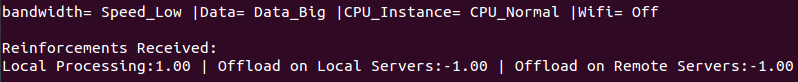
\includegraphics[width=5in]{RL_Local.png}
  \caption{Best Action: Local Processing}
  \label{fig:RL_Local}
\end{figure}
\begin{figure}[h!]
  \centering
  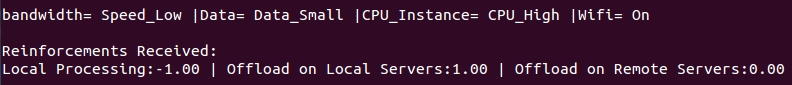
\includegraphics[width=5in]{RL_offload_Local.png}
  \caption{Best Action: Offload on Local servers, Second best action: Offload on remote Server}
  \label{fig:RL_offload_Local}
\end{figure}
\begin{figure}[h!]
  \centering
  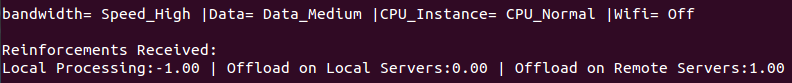
\includegraphics[width=5in]{RL_offload_Remote.png}
  \caption{Best Action: Offload on Remote servers, Second best action: Offload on Local Server}
  \label{fig:RL_offload_Remote}
\end{figure}
%%%%%%%%%%%%%%%%%%%%%%%%%%%%%%%%%%%%%%%%%%%%%%%%%%%%%%%%%%%%%%%%%%%%%
\subsection{Scenario 2}
In the previous scenario we do not have multiple steps of reinforcements. RL also works in the situation where we have different stages and steps for example in a tic-tac-toe game or even chess. So the previous scenario does not exploit the multiple step option available with RL.\par
In this second scenario we can envision a situation where we need to further choose from right actions after we have decided whether to offload or not, for example after offloading we might lower the CPU frequency rate of the device to lower the battery consumption, or after offloading we can choose for a specific service that is being offered by the Commercial server provider to get the best of what is available with us and so on.\par
We can also add time factor as a parameter as sometimes it is seen that the internet speed or performance varies depending which part of day we are using it (because of varying load of users).
%%%%%%%%%%%%%%%%%%%%%%%%%%%%%%%%%%%%%%%%%%%%%%%%%%%%%%%%%%%%%%%%%%%%%%

\section{Discussion}
Machine learning algorithms such as Reinforcement Learning with Neural Network and others requires multiple trials for a well trained $Q$ functions which might run into hundreds or thousands of iterations.
For the compute intensive applications the offloading is beneficial as we have seen in \cite{kumar2010cloud}. For example if we
want to train a neural network for a smartphone device which has thousands of iterations, we
can offload he training of Q function on the Cloud, and use the trained function for the decision making.

%%%%%%%%%%%%%%%%%%%%%%%%%%%%%%%%%%%%%%%%%%%%%%%%%%%%%%%%%%%%%%%%%%%%%%
\section{Next Steps}
It will be interesting to use Neural Network with Reinforcement Learning, right now I am working on a Python code which will use Neural Network to train the $Q$ function that we studied in this report.\par
I am also working on an algorithm which uses QDA or LDA Classification techniques for the offloading decision engine. I believe Classification can be useful when applied on the useful data obtained from Reinforcement Learning method, as it requires much lesser calculations than RL, so it will be more efficient.
%%%%%%%%%%%%%%%%%%%%%%%%%%%%%%%%%%%%%%%%%%%%%%%%%%%%%%%%%%%%%%%%%%%%%%
\section{Conclusion}
I have demonstrated some ways with which we can enhance the offloading process with the help of an offloading engine which uses Reinforcement Learning (In my previous report I had used Fuzzy Logic). I found Reinforcement learning is very exciting and promising when used in intuitive situations such as the one which is presented in this report where should be able to save battery power. \par
When the Machine Learning algorithms such as RL with Neural Network needs a lot of processing to train itself, at that time the smartphone-cloud coupling can prove useful as the device need not bother about big number of iterations, it can just offload the processing on cloud. \cite{flores2013adaptive}

%%%%%%%%%%%%%%%%%%%%%%%%%%%%%%%%%%%%%%%%%%%%%%%%%%%%%%%%%%%%%%%%%%%%%%

\bibliographystyle{plainnat}  % or plain, or many other possibilities
\bibliography{bibkrishna.bib}


\end{document}
